\documentclass[11pt,letter]{article}
\usepackage[margin=1in]{geometry}

\usepackage[english]{babel}
\usepackage[utf8]{inputenc}
\usepackage[T1]{fontenc}
\usepackage{stmaryrd}
\usepackage{footmisc}

\usepackage{csquotes}

\usepackage{mathrsfs}
\usepackage{amsmath}
\usepackage{amssymb}
\usepackage{bbm}
\usepackage{graphicx}
\usepackage{stackengine}
\usepackage{amsthm}
\usepackage{subcaption}

\usepackage{thmtools}
\usepackage{thm-restate}

\usepackage[colorinlistoftodos]{todonotes}
\usepackage[colorlinks=true, allcolors=blue]{hyperref}

\usepackage{amsfonts}
\usepackage{cleveref}


\usepackage{soul}
\newcommand{\ml}[1]{{\color{blue}{#1}}}
\newcommand{\nn}[1]{{\color{red}{#1}}}
\newcommand{\md}[1]{{\color{orange}{#1}}}




\newtheorem{theorem}{Theorem}[section]
\newtheorem{thm}[theorem]{Theorem}
\newtheorem{conjecture}[theorem]{Conjecture}
\newtheorem{lemma}[theorem]{Lemma}
\newtheorem{lm}[theorem]{Lemma}
\newtheorem{prob}[theorem]{Open Problem}
\newtheorem{corollary}[theorem]{Corollary}
\newtheorem{proposition}[theorem]{Proposition}
\newtheorem{claim}[theorem]{Claim}
\theoremstyle{remark}
\newtheorem*{definition}{Definition}
\newtheorem*{remark}{Remark}
\newtheorem*{recall}{Recall}

\newcommand{\binuparrow}{\mathbin{\uparrow}}
\newcommand{\T}{\text{Top}}
\newcommand{\B}{\text{Bot}}
\newcommand{\F}{\mathscr{F}}
\renewcommand{\L}{\mathcal{L}}    
\newcommand{\set}[1]{\left\{#1\right\}}

\def\rddots#1{\cdot^{\cdot^{\cdot^{#1}}}}


\usepackage{tikz}
\usetikzlibrary{fit,positioning,calc}


\newenvironment{prevproof}[2]{\noindent {\bf {Proof of {#1}~\ref{#2}:}}}{$\qed$\vskip \belowdisplayskip}

\newcommand{\bb}{\mathbb}
\DeclareMathOperator{\dist}{dist}

\title{$k$-Leaf Powers Cannot be Characterized by a Finite Set of Forbidden Induced Subgraphs for $k \geq 5$}
\date{ }
\author{
    Max Dupr\'e la Tour\thanks{McGill University: \texttt{maxduprelatour@gmail.com}} \and 
       Manuel Lafond\thanks{Universit\'e de Sherbrooke: \texttt{manuel.lafond@usherbrooke.ca}} \and 
  Ndiam\'e Ndiaye\thanks{McGill University. \texttt{ndiame.ndiaye@mail.mcgill.ca}} \and 
    Adrian Vetta\thanks{McGill University. \texttt{adrian.vetta@mcgill.ca}}
}

 



\begin{document}
\maketitle

\begin{abstract}
A graph $G=(V,E)$ is a $k$-leaf power if there is a tree $T$ whose leaves are the vertices of $G$ with the property that 
a pair of leaves $u$ and $v$ induce an edge in $G$ if and only if they are distance at most $k$ apart in $T$.
For $k\le 4$, it is known that there exists a finite set $\F_k$ of graphs such that the class $\L(k)$ of $k$-leaf power graphs is characterized as the set of strongly chordal graphs that do not contain any graph in $\F_k$ as an induced subgraph. 
We prove no such characterization holds for $k\ge 5$.
That is, for any $k\ge 5$, there is no finite set $\F_k$ of graphs such that $\L(k)$ is equivalent to the set of strongly chordal graphs that do not contain as an induced subgraph any graph in $\F_k$.
\end{abstract}

\section{Introduction}\label{sec:intro}

A fundamental question in graph theory concerns whether or not a graph $G=(V,E)$ can be represented (or approximated) by a simpler graph, for instance a tree $T$, while preserving the desired information from the original graph.  
The pairwise distances of $G$ often need to be summarized into sparser structures, with 
notable examples including \emph{graph spanners}~\cite{cohen2020light,ahmed2020graph,filtser2021graph,le2022near} and \emph{distance emulators}~\cite{thorup2006spanners,chang2022almost,van2022fast} which respectively ask for a subgraph of $G$ or for another graph that approximates the distances of $G$.
If the distance information to preserve only concerns ``close together'' versus ``far apart'' then this can take the following form:
given a graph $G$ and an integer $k$, does there exists a tree $T$ whose leaves are the vertices of $G$, such that distinct vertices $u$ and $v$ are adjacent in $G$  {\em if and only if} the distance $d_T(u,v)$ from $u$ to $v$ in $T$ is at most $k$?  If the answer is affirmative then $G$ is dubbed a $k$-{\em leaf power} of $T$ (and $T$ is dubbed a $k$-{\em leaf root} of $G$). 

The study of $k$-leaf powers and roots were instigated by Nishimura, Ragde and Thilikos~\cite{NISHIMURA200269}. On the applied side, these graphs are of significant interest in the field of computational biology with respect to {\em phylogenetic trees}, which aim to explain the distance relationships observed on available data between species, genes, or other types of taxa.  Indeed, $k$-leaf powers can be used to represent and explain pairs of genes that underwent a bounded number of evolutionary events in their evolution~\cite{long2020exact,hellmuth2020generalized}, or that have conserved closely related biological functions during evolution~\cite{lafond2014orthology}.
On the theory side, despite their simplicity, several fundamental graph theoretic problems concerning $k$-leaf powers remain open.
The purpose of this research is to resolve one such long-standing 
open problem. Specifically, we 
prove that the class $\L(k)$ of $k$-leaf power graphs cannot be characterized via a finite set of forbidden induced subgraphs for $k\ge 5$. In contrast, for $k\le 4$ such finite characterizations were previously shown to exist~\cite{DOM2004, BRANDSTADT2006,Brandstadt2008-4LP}.


\subsection{Background}
Let $\L(k)$ denote the class of all $k$-leaf power graphs, for $k \geq 2$. The class of all leaf power graphs is then
denoted by $\L = \bigcup_k \L(k)$.
The literature on leaf power graphs has primarily focused on two major themes. One, obtaining graphical characterizations for both the class $\L$ and the classes $\L(k)$, for fixed values of $k$. 
Two, designing efficient algorithms to recognize graphs that belong to these classes. 

Let's begin with the former theme. Here  important roles are played by chordal and strongly chordal graphs.
A graph is \emph{chordal} if every cycle of length four or more has a \emph{chord}, an edge connecting two non-consecutive vertices of cycle. A graph is \emph{strongly chordal} if it is chordal {\bf and} all its even cycles of length $6$ or more have an \emph{odd chord}, a chord connecting two vertices an odd distance apart along the cycle.
Now, it is known that every graph in $\L$ and $\L(k)$ is \emph{strongly chordal}.\footnote{In particular they do not contain, as induced subgraphs, chordless cycles of length greater than three, nor {\em sun graphs}.} To see this, first note that a leaf power graph is an induced subgraph of a power of a tree. Second,
note that trees are strongly chordal, and taking powers and induced subgraphs both preserve this property~\cite{raychaudhuri1992powers}).  
However, the reciprocal is not true: there exist strongly chordal graphs that are not leaf powers. The first such example was discovered by Brandst\"adt et al.~\cite{BRANDSTADT2010897}. Subsequently, six additional examples were identified by Nevries and Rosenke~\cite{nevries2016towards} who conjectured that any strongly chordal graph not containing any of these seven graphs as an induced subgraph is a leaf power. 
However, a weaker version of this conjecture, that there are only a finite number (rather than seven) of obstructions was
was disproved by Lafond~\cite{Lafond2017}. The author
constructed an infinite family of \emph{minimal} strongly chordal graphs that are not leaf powers (i.e., removing any vertex results in a leaf power). 

For fixed $k$, the conjecture that $\L(k)$ may be characterized by a finite set of obstructions remained open. 
Indeed, for $k\le 4$, the classes $\L(k)$ can be characterized as chordal graphs that do not contain any graph from $\F_k$ as induced subgraphs, where $\F_k$ is a finite set. Specifically:
\begin{itemize}
\item $k=2$: A graph is in $\L(2)$ {\em if and only if} it is a disjoint union of cliques. That is, $\L(2)$ is precisely the set of graphs that forbid $P_3$, the chordless path with three vertices, as an induced subgraph. Thus $|\F_2|=1$.
\item $k=3$: Dom et al.~\cite{DOM2004} gave the first characterization of $\L(3)$: a graph is in $\L(3)$ {\em if and only if} it is chordal and does not contain a bull, a dart or a gem as induced subgraph. Thus $|\F_3|=3$. Other characterizations of $\L(3)$ were later discovered~\cite{BRANDSTADT2006}
\item
$k=4$: Brandst\"adt, Bang Le and Sritharan~\cite{Brandstadt2008-4LP}
proved that a graph is in $\L(4)$ {\em if and only if} it is chordal and does not contain as induced subgraph one of a finite set $\F_4$ of graphs\footnote{Formally, they show that the set of basic 4-leaf power, where no two leaves of the leaf root share a parent, can be characterized by chordal graphs which do not have one of 8 graphs as induced subgraphs. $\F_4$ can be deduced from this set.}.
\end{itemize}
Given this, the aforementioned conjecture naturally arose: for every $k$, is the class $\L(k)$ equivalent to the set of chordal graphs that do not contain as induced subgraphs any of a finite set $\F_k$ of graphs? 

For $k=5$, Brandst\"adt, Bang Le and Rautenbach~\cite{BRANDSTADT20093843} proved this is true for a special subclass of $\L(5)$. Specifically, the \emph{distance hereditary}\footnote{A graph $G$ is distance hereditary if for all pairs of vertices $(u,v)$ in all subgraphs of $G$ either the distance is the same as in $G$ or there is no path from $u$ to $v$.} $5$-leaf power graphs are chordal graphs that do contain a set of $34$ graphs as induced subgraphs.
However, for the general case, they state
\begin{quote}
    ``{\em For $k\geq 5$, no characterization of $k$-leaf powers is known despite considerable effort. Even the characterization of $5$-leaf powers appears to be a major open problem.''~\cite{BRANDSTADT20093843}} 
\end{quote}
The contribution of this paper is to disprove the conjecture: for all $k\geq 5$, it is impossible to characterize the set of $k$-leaf powers as the set of chordal graphs which are $\F_k$-free for $|\F_k|$ finite. In fact, we show that even for the more restrictive class of strongly chordal graphs it is impossible to characterize the set of $k$-leaf powers as the set of strongly chordal graphs which are $\F_k$-free for finite $|\F_k|$. 

Let us conclude this section by discussing the second major theme
in this area, namely, efficient recognition algorithms.
The computational complexity of deciding whether or not a graph is in $\L$ is wide open.  
We remark, however, that some graphs in $\L$ have a {\em leaf rank} that is exponential in the number of their vertices, where the leaf rank of a graph $G$ is the minimum $k$ such that $G \in \L(k)$~\cite{LowerBoundsLR}.  The question of computing the leaf rank of subclasses of $\L$ in polynomial time was recently initiated in~\cite{le2023computing}.

For fixed values of $k$, though, progress has been made in designing polynomial-time algorithms for the $\L(k)$ recognition problem.  For $\L(2), \L(3)$ and $\L(4)$, this immediately follows from the above characterizations because $\F_2, \F_3$ and $\F_4$ are finite. 
In fact, all these three recognition problems can be solved in linear time; see \cite{BRANDSTADT2006,Brandstadt2008-4LP}.
Using a dynamic programming approach, Chang and Ko~\cite{Chang2007} described a linear-time algorithm for the $\L(5)$ recognition problem, and Ducoffe~\cite{ducoffe20194} proposed a polynomial-time algorithm for the $\L(6)$ recognition problem. Recently, Lafond~\cite{Lafond2023} designed a polynomial-time algorithm for the $\L(k)$ recognition problem, for any constant $k \geq 2$. 
The algorithm is theoretically efficient albeit completely impractical: the polynomial's exponent depends only on $k$ but is $\Omega(k \binuparrow\binuparrow k)$, that is, a tower of exponents $k^{k^{\rddots k}}$ of height $k$.  
We remark that the algorithm 
does not rely on specific characterizations of $k$-leaf power graphs aside from the fact that they are chordal. It appears difficult to significantly improve its running time without a better understanding of the graph theoretical structure of graphs in $\L(k)$.  Our work assists in this regard by improving our knowledge of $k$-leaf powers in terms of forbidden induced subgraphs.




\subsection{Overview and Results}
We now present an overview of the paper and our results.
In Section~\ref{sec:proof} we present our main theorem:
\begin{restatable}{theorem}{main}\label{thm:main}
    For $k\geq 5$, the set of $k$-leaf powers cannot be characterized as the set of strongly chordal graphs which are $\F_k$-free, where $\F_k$ is a finite set of graphs.
\end{restatable}

There we discuss the three types of gadgets we need. These gadgets can be combined to form an infinite family of pairwise incomparable graphs which are not $k$-leaf powers.
We prove the main theorem modulo three critical lemmas on the gadgets. 
In Section~\ref{sec:gadgets} we present proofs of the three critical lemmas.
Finally, in Section~\ref{sec:linear} we show how to modify our proof
to derive a similar theorem for \emph{linear $k$-leaf powers}:
\begin{restatable}{theorem}{linear}\label{thm:linear}
    For $k\geq 5$, the set of linear $k$-leaf powers cannot be characterized as the set of strongly chordal graphs which are $\F_k$-free where $\F_k$ is a finite set of graphs.
\end{restatable}
Here, a linear $k$-leaf power is a graph that has a $k$-leaf root which is the subdivision of a \emph{caterpillar}. We remark that that the class of linear leaf powers can be recognised in linear time, as shown by Bergougnoux et al.~\cite{Bergougnoux}.




\section{The Proof Modulo Three Critical Lemmas}\label{sec:proof}

In this section we prove our main theorem, Theorem~\ref{thm:main},
assuming the validity of three critical lemmas.
The proofs of these lemmas form the main technical contribution of the paper and are deferred to Section~\ref{sec:gadgets}.


\subsection{Preliminaries}
Before presenting the proof of Theorem~\ref{thm:main}, we present  
necessary definitions and notations.
Let's start with a formal definition of $k$-leaf powers. Let $G = (V,E)$ be a simple finite graph, and $k\geq 2$ be an integer. $G$ is called a $k$-\emph{leaf power} if there exists a tree $T$, known as a {\em $k$-leaf root of $G$}, with the following properties:
\begin{itemize}
    \item $V$ is the set of leaves of $T$.
    \item For any pair of vertices $u,v \in V$, there is an edge $uv \in E$ {\em if and only if} the $d_T(u,v) \leq k$.
\end{itemize}
Here $d_T$ is the distance metric induced by the tree $T$ when two adjacent vertices are a distance of~$1$ apart.
To simplify the notation, we will use $d$ instead of $d_T$ when the context is clear. We will use the notation $\dist_G$ to denote distance within the graph $G$ and thus distinguish it from the distance $d_T$ induced by a leaf root $T$.


 


\subsection{The Proof of the Main Theorem}

To prove Theorem~\ref{thm:main}, for any $k\ge 5$, we will construct a collection of arbitrarily large strongly chordal graphs that are \emph{minimal non }$k$\emph{-leaf powers}. Specifically, these graphs have the property that any ``strict'' induced subgraph is a $k$-leaf power.

To accomplish this goal, we fix $k\ge 5$. We then begin by designing a graph $H_n$, for all $n\geq 0$,
built using three gadget graphs joined in series. First will be the {\em top gadget} and last the {\em bottom gadget}. In between will be exactly $n$ copies of the 
{\em interior gadget}.
We denote these gadget graphs by $\T, \B$ and $I$,
respectively. These gadget graphs will satisfy a set
of critical properties. To formalize these properties we require the following definition.
Given a graph $G=(V,E)$ and $T$ a $k$-leaf root of $G$. For $v\in V$, let $m_T(v)=\min_{u\in V\setminus \{v\}} d_T(u,v)$. That is, $m_T(v)$ is the shortest distance in the tree $T$ from the leaf $v$ to any other leaf $u$. 

The aforementioned properties of $\T, \B$ and $I$ are stated in the subsequent three critical lemmas.

\begin{restatable}{lemma}{top}
    \label{lem:top}
For all $k\geq 4 $, there exists a gadget graph $\T$ that contains a vertex $t\in V(\T)$ such that:
\begin{enumerate}
        \item For any $k$-leaf root $T$ of $\T$, $m_{T}(t) = 3$.
        \item There exists a $k$-leaf root $T_{\T}$ of  $\T$.
    \end{enumerate}
\end{restatable}

\begin{restatable}{lemma}{bot}\label{lem:bottom}
For all $k\geq 4$, there exists a gadget graph $\B$ that contains a vertex $b \in V(\B)$ such that:
\begin{enumerate}
        \item For any $k$-leaf root $T$ of $\B$, $m_T(b) \leq k-1$.
        \item There exists a $k$-leaf root $T_{\B}$ such that $m_{T_{\B}}(b) = k-1$
\end{enumerate}
\end{restatable}   
\begin{restatable}{lemma}{ind}\label{lem:induction}
For all $k\geq 5$, there exists a gadget graph $I$ that contains two distinct vertices $t_I,b_I\in V(I)$ such that:
\begin{enumerate}
        \item For all $k$-leaf roots $T$ of $I$, $m_T(t_I)\geq k\Longrightarrow m_T(b_I)=3$.
        \item There exists a $k$-leaf root $T_I$ of $I$ such that $m_{T_I}(t_I)=k$ and $m_{T_I}(b_I)=3$.
        \item There exists a $k$-leaf root $R_I$ of $I$ such that $m_{R_I}(t_I)=k-1$ and $m_{R_I}(b_I)=4$.
    \end{enumerate}    
\end{restatable}

We will prove the existence of gadget graphs
$\T, \B$ and $I$ required to verify the three lemmas in Section~\ref{sec:gadgets}.
For the rest of the section, we will assume these lemmas and use them to prove our main result.

\begin{figure}[h!]
    \centering
    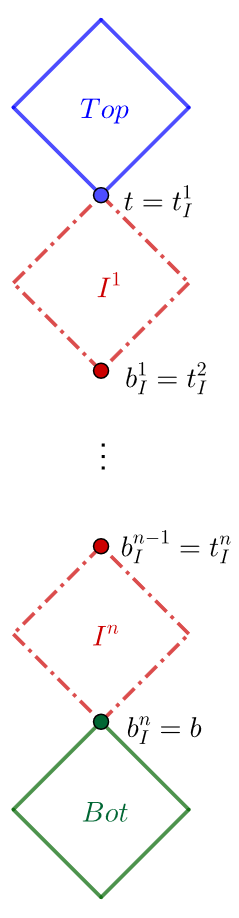
\includegraphics[height=10cm]{ConstructionHn.png}
    \caption{The construction of $H_n$}\label{fig:Hn}
\end{figure}

First, as alluded to above, we then combine our three gadgets to create an intermediary graph $H_n$. In particular, $H_n$ is the graph obtained by connecting in series one copy of $\T$,
then $n$ copies of $I$: $I^1, \dots, I^n$ and finally one copy of $\B$.  
This construction is illustrated in \Cref{fig:Hn}.
The vertices $t_I$ and $b_I$, mentioned in Lemma~\ref{lem:induction}, of the $j$-th copy $I^j$ are denoted $t^j_I$ and $b^j_I$, respectively.
Notice that to connect the gadgets within $H_n$, we identify the vertices described in Lemmas~\ref{lem:top}, \ref{lem:bottom}, and \ref{lem:induction} as follows. We identify $t$ with $t^1_I$, for all $j < n$, $b^j_I$ with $t^{j+1}_I$, and finally, $b^n_I$ with $b$. As a special case when $n = 0$, the graph $H_0$ is obtained by taking $\T$ and $\B$ and identifying $t$ with $b$.

In order to prove Theorem~\ref{thm:main} we must study the structure of $H_n$. We denote by $H_n - \T$ (resp. $H_n - \B$) the graph obtained from $H_n$ by deleting the top gadget $\T$ (resp. the bottom gadget $\B$), i.e. removing all vertices of $\T$ (resp. $\B$) except for the common vertex $t = t_I^1$ (resp. $b = b_I^n$). Of importance is the next lemma.
\begin{lemma}\label{lem:Hn}
    The graph $H_n$ has the following properties:
    \begin{enumerate}
        \item $\dist_{H_n}(b,t) \geq n$. \label{cond:increasing}
        \item $H_n$ is strongly chordal. \label{cond:Str-Chordal}
        \item $H_n - \T$ and $H_n - \B$ are both $k$-leaf powers. \label{cond:Top/Bot}
        \item $H_n$ is not a $k$-leaf power. \label{cond:not-LP}
        \end{enumerate}
\end{lemma}
\begin{proof}\textcolor{red}{TOPROVE 0}\end{proof}

As stated $H_n$ is an intermediate graph in proving the main result. 
We will actually show the existence
of an induced subgraph $G_{k,n}$ of $H_n$
that is strongly chordal and minimal non $k$-leaf power.
More precisely, we have the following lemma.

\begin{lemma}\label{lem:Gn}
    For all $k\geq 5$ and $n\geq 0$, there exists a graph $G_{k,n}$ such that:
\begin{enumerate}
    \item $G_{k,n}$ is strongly chordal and contains at least $n$ vertices.
    \item $G_{k,n}$ is not a $k$-leaf power.
    \item If $G\neq G_{k,n}$ is an induced subgraph of $G_{k,n}$ then $G$ is a $k$-leaf power.
\end{enumerate}
\end{lemma}
\begin{proof}\textcolor{red}{TOPROVE 1}\end{proof}

Our main result follows directly from Lemma~\ref{lem:Gn}

\begin{proof}\textcolor{red}{TOPROVE 2}\end{proof}





\section{The Gadget Graphs}\label{sec:gadgets}

So we have proven the main theorem modulo the three critical lemmas.
Recall to prove these lemmas we must construct the appropriate three gadget graphs, namely $\T$, $\B$ and $I$.
We present these constructions and give formal proofs of 
Lemmas~\ref{lem:top},~\ref{lem:bottom} and~\ref{lem:induction} in this section.

We start with a general observation. In a tree $T$, if a pair of leaves are a distance of~$2$ apart, they share the same parent. Consequently, their distances to every other leaf are identical. A consequence of this is that if two vertices are not connected by an edge, or if they have different neighborhoods in a graph, they must be at a distance of at least $3$ in any leaf root of that graph. In the gadgets we describe in this section, any two vertices connected by an edge always have distinct neighborhoods. Therefore, we assume that for any pair of vertices $x$ and $y$ and any leaf root $T$, we have $d_T(x, y) \geq 3$.


\subsection{The Top Gadget}\label{sec:top}

We begin by showing the existence of an appropriate top gadget, $\T$.

\top*
\begin{proof}\textcolor{red}{TOPROVE 3}\end{proof}

\begin{figure}[!h]
    \centering
    \begin{subfigure}{0.45\textwidth}
        \centering
        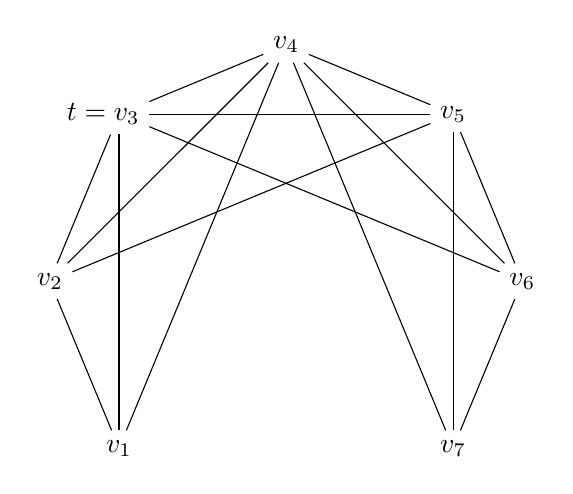
\begin{tikzpicture}
\node (P1) at (225:3) {$v_1$};
            \node (P2) at (180:3) {$v_2$};
            \node (P3) at (135:3) {$\hspace{-4mm}t=v_3$};
            \node (P4) at (90:3) {$v_4$};
            \node (P5) at (45:3) {$v_5$};
            \node (P6) at (0:3) {$v_6$};
            \node (P7) at (315:3) {$v_7$};
            \draw (P1) -- (P2) -- (P3) -- (P4) -- (P5) -- (P6) -- (P7);
            \draw (P1) -- (P3) -- (P5) -- (P7);
            \draw (P2) -- (P4) -- (P6);
            \draw (P1) -- (P4) -- (P7);
            \draw (P2) -- (P5);
            \draw (P3) -- (P6);
        \end{tikzpicture}
\end{subfigure}
    \quad
    \begin{subfigure}{0.45\textwidth}
        \centering
        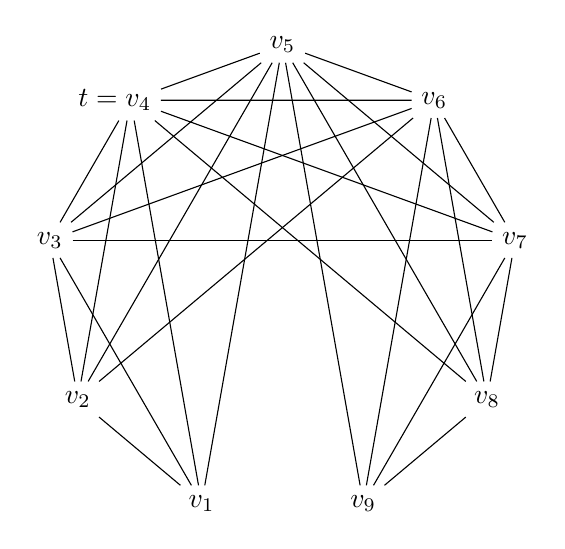
\begin{tikzpicture}
\node (P1) at (250:3) {$v_1$};
            \node (P2) at (210:3) {$v_2$};
            \node (P3) at (170:3) {$v_3$};
            \node (P4) at (130:3) {$\hspace{-4mm}t=v_4$};
            \node (P5) at (90:3) {$v_5$};
            \node (P6) at (50:3) {$v_6$};
            \node (P7) at (10:3) {$v_7$};
            \node (P8) at (330:3) {$v_8$};
            \node (P9) at (290:3) {$v_9$};
\draw (P1) -- (P2) -- (P3) -- (P4) -- (P5) -- (P6) -- (P7) -- (P8) -- (P9);
            \draw (P1) -- (P3) -- (P5) -- (P7) -- (P9);
            \draw (P2) -- (P4) -- (P6) -- (P8);
            \draw (P1) -- (P4) -- (P7);
            \draw (P2) -- (P5) -- (P8);
            \draw (P3) -- (P6) -- (P9);
            \draw (P1) -- (P5);
            \draw (P2) -- (P6);
            \draw (P3) -- (P7);
            \draw (P4) -- (P8);
            \draw (P5) -- (P9);
        \end{tikzpicture}
\end{subfigure}
\caption{The Top Gadget for $k=5$ and $k=6$.}
    \label{fig:top-gadget}
\end{figure}


\subsection{The Bottom Gadget}\label{sec:bot}

Next, we construct the bottom gadget, $\B$. 
A key technical tool we require is the {\em 4-Point Condition}. 
This is the following classical characterization of tree metrics. 
\begin{theorem}[4-Point Condition]\label{thm:4-PC} \cite{BUNEMAN197448}
    Let $d$ be a distance on a finite set $V$, then there exists a tree $T$ whose leaves are $V$ such that $\forall u,v\in V$ $d_T(u,v)=d(u,v)$ if and only if the following condition is true for all $(u,v,w,t)\in V$:
    \[d(u,v)+d(w,t)\leq \max\set{d(u,w)+d(v,t),d(v,w)+d(u,t)}.\]
\end{theorem}

Our bottom gadget $\B$ will simply be a {\em diamond}, the complete graph on 4 vertices minus one edge.
Consequently, we begin by proving the following corollary of the $4$-Point Condition when applied to a diamond.

\begin{corollary}\label{cor:diamond}
    In any $k$-leaf root $T$ of a diamond with vertex set $\set{b,v_1,v_2,v_3}$ where $(v_1,v_3)\notin E$, $d(b,v_2)\neq k$.
\end{corollary}

\begin{proof}\textcolor{red}{TOPROVE 4}\end{proof}

Corollary~\ref{cor:diamond} allows us to prove our critical lemma for the bottom gadget.

\bot*

\begin{proof}\textcolor{red}{TOPROVE 5}\end{proof}



\subsection{The Interior Gadget}\label{sec:int}

Lastly, we have the most complex construction, that of 
the interior gadget, $I$. 
Now we require the following lemma which, again, is a consequence of the 4-Point Condition.

\begin{lemma}\label{lem:closer}
    If $d(t,x_1)\leq \min\set{d(t,x_2),d(t,x_3)}$ and $d(y,x_1)>\max\set{d(y,x_2),d(y,x_3)}$, then:
    \[d(t,x_1)+d(x_2,x_3)<d(t,x_2)+d(x_1,x_3)=d(t,x_3)+d(x_1,x_2)\]
\end{lemma}

\begin{proof}\textcolor{red}{TOPROVE 6}\end{proof}

We will also use the following simple lemma:

\begin{lemma}\label{lem:even}
    For any 3 leaves $u,v,w$ of a tree, $d(u,v)+d(u,w)+d(v,w)$ is even.
\end{lemma}

\begin{proof}\textcolor{red}{TOPROVE 7}\end{proof}

We now have all the tools needed to prove our critical lemma for the interior gadget.


\ind*

Before proving this lemma, let's discuss the requirement that $k\ge 5$.
First observe that no such graph can exist for $k\leq 2$ because if $m_T(b_I)=3$ then $b_I$ is an isolated vertex in $I$. Thus its distance to other leaves does not matter as long as it's large enough, so the lemma could not hold.
Similarly, if $k=3$, the existence of a $3$-leaf root $T_I$ implies that $b_I$ is not an isolated vertex in $I$. But the existence of a $3$-leaf root $R_I$ implies that $b_I$ is an isolated vertex, a contradiction. 
Finally, for $k=4$, while there is no direct simple proof that the statement does not hold for any graph, 
the existence of a characterization of $4$-leaf powers implies that no such graph can exist.

\begin{proof}\textcolor{red}{TOPROVE 8}\end{proof}
With our three critical lemmas proven, the main theorem now holds
by the method shown in Section~\ref{sec:proof}.

\section{Linear Leaf Powers}\label{sec:linear}

A {\em caterpillar} is a graph which has a central path and a set of leaves whose neighbor is on the central path. A graph is said to be a \textit{linear leaf power} if it has a leaf root which is the subdivision of a caterpillar. Such a leaf root is called a \textit{linear leaf root}~\cite{Bergougnoux}.

Our results apply not only to general leaf powers but also to this variant. Indeed, even if we restrict to having a subdivision of a caterpillar as a leaf root, it is impossible to get a simple forbidden
subgraph characterization of linear $k$-leaf powers for $k \geq 5$.

\begin{theorem}\label{thm:caterpillar}
    For $k\geq 5$, the set of linear $k$-leaf powers cannot be written as the set of strongly chordal graphs which are $\F_k$-free where $\F_k$ is a finite set of graphs.
\end{theorem}

As in the general case, we prove this using three gadgets. However, we must now add a condition to ensure that merging the gadgets preserves having a subdivision of a caterpillar as a leaf root.

\begin{lemma}\label{lem:top-caterpillar}
For all $k\geq 5$ there exists a gadget graph $\T$ that contains a vertex $t\in V(\T)$ such that:
\begin{enumerate}
        \item For any linear $k$-leaf root $T$ of $\T$, $m_{T}(t) = 3$.
        \item There exists a linear $k$-leaf root $T_{\T}$ of  $\T$ where $t$ is a neighbor of the last node of the central path.
    \end{enumerate}
\end{lemma}

\begin{lemma}\label{lem:bottom-caterpillar}
For all $k\geq 5$ there exists a gadget graph $\B$ that contains a vertex $b \in V(\B)$ such that:
\begin{enumerate}
        \item For any linear $k$-leaf root $T$ of $\B$, $m_T(b) \leq k-1$.
        \item There exists a linear $k$-leaf root $T_{\B}$ such that $m_{T_{\B}}(b) = k-1$ where $b$ is a neighbor of the last node of the central path.
\end{enumerate}
\end{lemma}

\begin{lemma}\label{lem:induction-caterpillar}
For all $k\geq 5$ there exists a gadget graph $I$ that contains two distinct vertices $t_I,b_I\in V(I)$ such that:
\begin{enumerate}
        \item For all linear $k$-leaf roots $T$ of $I$, $m_T(t_I)\geq k\Longrightarrow m_T(b_I)=3$.
        \item There exists a linear $k$-leaf root $T_I$ of $I$ such that $m_{T_I}(t_I)=k$ and $m_{T_I}(b_I)=3$ where $b$ and $t$ are neighbors of the first and last node of the central path respectively.
        \item There exists a linear $k$-leaf root $R_I$ of $I$ such that $m_{R_I}(t_I)=k-1$ and $m_{R_I}(b_I)=4$ where $b$ and $t$ are neighbors of the first and last node of the central path respectively.
    \end{enumerate}    
\end{lemma}

Merging the gadgets is identical to before except that we now use the condition that, in each gadget, $t$ and/or $b$ are neighbors of the extremal vertices of the central path. This means when merging the gadgets using the parent of these vertices, we merge the central paths by their endpoint to create a longer path, ensuring we produce another caterpillar subdivision.

We can verify that Lemma~\ref{lem:bottom-caterpillar} follows from Lemma~\ref{lem:bottom} and Lemma~\ref{lem:induction-caterpillar} follows from Lemma~\ref{lem:induction}, as our constructions for the interior gadget and the Bottom Gadget used for the general case satisfy the properties needed, namely the leaf root used in the proofs are subdivisions of caterpillars with the required vertices connected to the extremal vertices of the central path. On the other hand, the graph used to construct the Top Gadget does not satisfy this property\footnote{The Top Gadget for the case of general $k$-leaf powers is a caterpillar but the vertex $t$ used is not connected to an extremal vertex of the central path.}; so we need to construct a new graph for $\T$.

\begin{proof}\textcolor{red}{TOPROVE 9}\end{proof}
We remark that this result does not immediately imply that there is no characterization for the entire class of linear leaf powers using chordal graphs and a finite number of forbidden induced subgraphs.
We have proven that such a characterization is impossible for each $k\geq 5$, but not necessarily for the union over all $k$. It was proved by Bergougnoux et al.~\cite{Bergougnoux} that linear leaf powers are also co-threshold tolerance. Further work on this could include verifying whether co-threshold tolerance graphs can be characterized using a finite number of obstructions.
Furthermore, it is worth noting that, despite Lemma~\ref{thm:caterpillar}, linear leaf powers are recognizable in polynomial time~\cite{Bergougnoux}. 

\section{Acknowledgements}

We would like to thank the Montreal Game Theory Workshop for helping bring together our research group.


\section{Conclusion}
We have shown that $k$-leaf powers require a deeper characterization than strong chordality with a finite set of forbidden induced subgraphs. Several directions  to explore remain in order to gain a more comprehensive understanding of $k$-leaf power graphs.
First, is it possible to construct and/or characterize minimal, strongly chordal graphs that are not $k$-leaf powers?  We were able to construct graphs $H_n$ that \emph{contain} such minimal examples as induced subgraphs; but we did not construct those examples explicitly.
Following this line of reasoning, it may be possible to characterize $k$-leaf powers as strongly chordal graphs that also forbid an additional infinite, but easy-to-describe family of forbidden subgraphs. A famous example of this are interval graphs, which are the chordal graphs containing no asteroidal triples~\cite{LB62}.

Second, are there relevant subclasses of $k$-leaf powers that can be characterized by strong chordality and a finite set of forbidden induced subgraphs?  For example, the $k$-leaf powers whose $k$-leaf roots admit a subdivision of a star should be easy enough to characterize. What about subdivisions of a tree with a small number, say two or three, of non-leaf vertices?   
One may also consider the $k$-leaf powers of caterpillars (not subdivided). Based on the midpoint arguments of Brandstädt et al.~\cite[Theorem 6]{BRANDSTADT2010897}, it would appear that, for even $k$, these coincide with the unit interval graphs whose intervals have length $k-2$ and integer endpoints.  Such (twin-free) graphs were shown to admit a finite set of forbidden induced subgraphs in~\cite{duran2015unit}. If this characterization extends to caterpillar $k$-leaf powers, this would show that taking subdivisions is necessary for our result on caterpillar graphs. 
It may also be interesting to characterize $k$-leaf powers for other graph classes that are known to be contained in $\L$; for instance, $k$-leaf powers that are also ptolemaic graphs, interval graphs, rooted directed path graphs, and others. 




 







\bibliographystyle{plain}
\bibliography{biblio}

\end{document}
